\documentclass[ngerman, 11pt]{scrreprt}

\usepackage{etoolbox}
\newtoggle{FOLIE}
\toggletrue{FOLIE}

%Grundlegendes: Schriftarten, deutsche Silbentrennung, Umlaute,...
\usepackage[utf8]{inputenc} 
\usepackage[T1]{fontenc}
\usepackage[ngerman]{babel}
\usepackage{lmodern}
\renewcommand*\familydefault{\sfdefault} %% Only if the base font of the document is to be sans serif
%\usepackage{times}
%\usepackage{bookman}
%\usepackage{palatino}

% fuer Stichwortverzeichnis
%\usepackage{makeidx}
% Stichwortverzeichnis erstellen
%\makeindex

%Kolumnentitel
\usepackage{fancyhdr}
\pagestyle{fancy}
% Definition der Kolumnentitel für den fancy-Style
\fancyhead{} %clear all header fields
\fancyhead[RO]{ %
	\iftoggle{FOLIE}{
		% keine Seitenzahl auf Folien
	}{%
		\begin{tikzpicture}[]
		\fill [CadetBlue!70!green] (0,0) circle (0.25cm); %ursprünglich gray!50!white
		\fill [CadetBlue!70!green] (-0.25,0) rectangle (0.25,-0.3);
		\draw [thick, gray!50!white] (-0.1,-0.3) -- (-0.1,-0.4);
		\draw [thick, gray!50!white] (0.1,-0.3) -- (0.1,-0.5);
		\node at (0,-0.05) {\sffamily \bfseries\thepage};
		\end{tikzpicture}
	}
} %Seitenzahl auf ungeraden (odd) Seiten rechts, auf geraden (even) links (Titelseite zählt mit)
\fancyhead[LE]{%
	\iftoggle{FOLIE}{%
		% keine Seitenzahl auf Folien
	}{%
		\begin{tikzpicture}[]
		\fill[CadetBlue!70!green] (0,0) circle (0.25cm);
		\fill [CadetBlue!70!green] (-0.25,0) rectangle (0.25,-0.3);
		\draw [thick, gray!50!white] (-0.1,-0.3) -- (-0.1,-0.5);
		\draw [thick, gray!50!white] (0.1,-0.3) -- (0.1,-0.4);
		\node at (0,-0.05) {\sffamily \bfseries\thepage};
		\end{tikzpicture}
	}
}
\fancyhead[LO]{%
	\iftoggle{FOLIE}{%
		\href{https://creativecommons.org/licenses/by-nc-sa/4.0/deed.de}{
\includegraphics[width=0.12\textwidth]{../pics/cc-by-nc-sa.png}~Voß}
	}{%
		\href{https://creativecommons.org/licenses/by-nc-sa/4.0/deed.de}{
\includegraphics[width=0.12\textwidth]{./pics/cc-by-nc-sa.png}~Voß}
	}
}
\fancyhead[RE]{%
	\iftoggle{FOLIE}{%
		\href{https://creativecommons.org/licenses/by-nc-sa/4.0/deed.de}{Voß~
\includegraphics[width=0.12\textwidth]{../pics/cc-by-nc-sa.png}}	
	}{%
		\href{https://creativecommons.org/licenses/by-nc-sa/4.0/deed.de}{Voß~
\includegraphics[width=0.12\textwidth]{./pics/cc-by-nc-sa.png}}
	}
}
\fancyhead[C]{\sffamily Arduino Skript}
\fancyfoot{} %clear all footer fields
% Die ersten Seiten eines Kapitels stellen automatisch den Seitenstil auf plain um. Daher wird der Seitenstil plain hier umdefiniert
\fancypagestyle{plain}{%
	\fancyhf{} %clear header und footer
	\renewcommand{\headrulewidth}{0pt}
	\renewcommand{\footrulewidth}{0pt}
}
\renewcommand{\headwidth}{\textwidth}



%Schriften/Mathe
\usepackage{amsmath}
\usepackage{amssymb}
\usepackage{amsfonts}
\usepackage{amsthm}

%Einheiten
\usepackage[separate-uncertainty=true]{siunitx} %Angabe im Befehl durch \SI{Wert(Fehler)}{Einheit}, Ausgabe als (Wert \pm Fehler) Einheit
\sisetup{locale=DE}

%Mehrspaltige Listen
\usepackage{multicol}

%Bilder
\usepackage[table,svgnames]{xcolor}
\usepackage{graphicx}
\usepackage{float}
\usepackage[footnotesize, indention=0cm, labelsep=space, textformat=simple]{caption}
\captionsetup[wrapfigure]{name=\textbf{B}} %Die Bildunterschriften für alle wrapfigures bekommen den Namen B. statt Abbildung
\captionsetup[figure]{name=\textbf{B}}

\usepackage{pgf,tikz,pgfplots}
\usepackage{mathrsfs}
\usetikzlibrary{arrows,arrows.meta}
\usetikzlibrary{intersections}
\usetikzlibrary{shadows}
\usetikzlibrary{automata, positioning}
\usepackage{calc} % ermöglicht es, für Längen u.ä. Rechnungen anzugeben wie \marginparsep+\marginparwidth
\usepackage{wrapfig}
\usepackage{eso-pic}
\usepackage{subfig}

%Tabellen
\usepackage{booktabs} % Basispaket für Tabellen
\usepackage{array} % Basispaket für Tabellen
\usepackage{tabu} % Hauptpaket, um Tabellen flexibel zu erstellen -> diese Dokumentation lesen // einige Befehle lassen sich nicht richtig benutzen und ich weiß nicht, woran das liegt...


%Rahmen
\usepackage{tcolorbox}
\tcbuselibrary{skins}
\tcbuselibrary{breakable}
		
%einfachere Anpassung von Listen
\usepackage{enumitem} 
	
%Fußnoten
\usepackage[bottom,hang]{footmisc}

%erweiterte Schleifen und Abfragen
\usepackage{xargs} %für mehrere optionale Argumente in eigenen Makros
\usepackage{ifthen} %für den whiledo Befehl

%Zitate
\usepackage{csquotes}


%Zum Einfügen von pdf Dokumenten mit \includepdf[options]{datei.pdf}
\usepackage[final]{pdfpages}
\includepdfset{pages=-,noautoscale}
	
\usepackage[twoside, top=2cm, outer=2.6cm, inner=2.6cm, % inner und outer sind aus irgendeinem Grund vertauscht
marginparwidth=2cm, marginparsep=0.3cm,% Die Breite für die Marginalien (Randbemerkungen) auf der rechten Seite
bottom=2cm, footskip=24pt, %Abstand zwischen Textboden und Fußzeilenboden
includefoot, includehead%
]{geometry}
\usepackage[strict]{changepage} % für lokales Überschreiben der Maße, damit man in den Rand schreiben kann (bei breiten Abbildungen z.B.)


\usepackage{setspace}
\usepackage{listings} %Zur Darstellung von Code
\lstset{backgroundcolor=\color{gray!15}, keywordstyle=\bfseries, commentstyle=\color{gray!80}, basicstyle=\ttfamily, identifierstyle=, stringstyle=\color{red!60!yellow}, emphstyle=\color{blue!60!green}, numbers=left, numberstyle=\tiny, stepnumber=2, numbersep=5pt}
\lstdefinestyle{Arduino}{%
	morekeywords={Serial, Servo},% define keywords
	morecomment=[l]{//},%             treat // as comments
	morecomment=[s]{/*}{*/},%         define /* ... */ comments
	emph={setup, loop, digitalWrite, digitalRead, analogWrite, analogRead, delay, print, println, pinMode},%        keywords to emphasize
	morestring=[b]",
}
\usepackage{blindtext}

% Einfügen von Meta-Daten in das PDF-Dokument
%\usepackage{hyperxmp}
\usepackage{xmpincl}

\usepackage[unicode]{hyperref}

\hypersetup{%
colorlinks=true, linkcolor=red!60!black,%Farbe für normale LInks
citecolor=green!60!black,%Farbe für Bibliographie-Links
filecolor=blue!60!black, %Farbe für Links zu lokalen Dateien
urlcolor=magenta!60!black,%Farbe für Links zu Internetadressen
pdfhighlight=/O,%Links werden gehighlighted, wenn man darauf geht, indem sie unterstrichen (outlined) werden
pdfnewwindow=true,%Links zu PDF-Dokumenten werden in neuem Fenster geöffnet
%XMP-Daten:
pdfauthor={Sebastian Voß},%
pdflang={de},%
pdftitle={Wahlpflichtfach Arduino},%
pdfsubject={Skript zur Einführung in Elektronik und Programmierung mit dem Arduino},%
%pdfcopyright={Dieses Werk ist lizenziert unter einer Creative Commons Namensnennung - Nicht-kommerziell - Weitergabe unter gleichen Bedingungen 4.0 International Lizenz},%
%pdflicenseurl={http://creativecommons.org/licenses/by-nc-sa/4.0/},%
%pdfurl={https://el-voss.de}
}


%Einfügen von Dateien (zusätzliche Arbeitsblätter, Folien,...)
\usepackage{attachfile2}
\attachfilesetup{author=Voß, color=0 0 .4}

%Symbole

% Symbol: Pfeil zum Zurückspringen
\newcommand{\zurueck}{%
	\begin{tikzpicture}[scale=0.15]
%	\fill [gray!40] (0,0) circle [radius=1.5];
	\draw [thick, -{>[length=3pt, width=5pt]}] (-0.6,0.6) arc [start angle=-230, end angle=100, radius=1] -- ++(-0.1,0);
	\end{tikzpicture}
}

%Symbol: Werkzeug
\newcommand{\werkzeug}{%
	\begin{tikzpicture}[scale=0.1, rotate=45]
%	\filldraw [fill=white, draw=black] (3,0) circle [radius=4cm];
	\path [thick, fill=gray, draw=black] (3.5,0.5) -- (0,0.5) arc [start angle=90, end angle=270, radius=0.5] (0,-0.5) -- (3.5,-0.5) -- (3.8,0) -- (3.5,0.5);
	\path [thick,draw=black, fill=gray] (3.5,-0.5) ++(1,0.5) ++(206.57:1.118) arc (206.57:315:1.118) -- ++(-0.9,0) -- (3.8,0) ++ (0.7,0) ++(-206.57:1.118) arc (-206.57:-315:1.118) -- ++(-0.9,0) -- (3.8,0);
	\draw [very thick, gray] (3.5,-0.5) -- (3.8,0) -- (3.5,0.5);
	\fill [gray!50, rounded corners=1] (0.3,0.25) rectangle (3.2,0.3);
	\fill [gray!50, rounded corners=1] (0.3,-0.25) rectangle (3.2,-0.3);
	\end{tikzpicture}
}

%Symbol: Drucker
\newcommand{\drucker}{%
	\begin{tikzpicture}[scale=0.2]
		\draw (0.5,0.5) rectangle (1.5,1.8);
		\foreach \x in {1.2,1.4,1.6}	
		\draw (0.6,\x) -- (1.4,\x);
		\draw [rounded corners=0.5pt, fill=gray!80!black] (0,0) rectangle (2,1);
	\end{tikzpicture}
}

%Symbol: Video
\newcommand{\video}{%
	\begin{tikzpicture}[scale=0.2]
		\draw [rounded corners=3pt, fill=gray!20] (0,0) rectangle (3,2);
		\draw [fill=gray] (1,0.5) -- (1,1.5) -- (2,1) -- (1,0.5);
	\end{tikzpicture}
}

%Symbol: Präsentationsfolie
\newcommand{\folie}{%
	\begin{tikzpicture}[scale=0.17]
	\draw [rounded corners=1pt,thick] (0,0) rectangle (3,2);
	\draw [rounded corners=1pt,fill=gray!30] (0.3,0.3) rectangle (1.3,1.6);
	\draw [rounded corners=1pt,fill=gray!30] (1.7,0.3) rectangle (2.7,1.6);
	\draw [thick] (1.1,-0.4) -- (1.5,0) -- (1.9,-0.4);
	\draw [fill=gray] (-0.2,1.8) rectangle (3.2,2.1);
	\end{tikzpicture}
}

%Symbol: Internetlink
\newcommand{\wlan}{%
	\begin{tikzpicture}[scale=0.5]
		\fill[black] (1mm,1mm) circle [radius=1mm];
		\draw [ultra thick] (0.4,0) arc [start angle=0, end angle=90, radius=4mm];
		\draw [ultra thick] (0.6,0) arc [start angle=0, end angle=90, radius=6mm];
		\draw [ultra thick] (0.8,0) arc [start angle=0, end angle=90, radius=8mm];
	\end{tikzpicture}
}

%Symbol: Ausrufezeichen
\newcommand{\ausrufezeichen}{%
	\begin{tikzpicture}[scale=0.8]
	\fill[gray!70] (0,0) circle [radius=1mm];
	\fill[gray] (0,0.15) -- (0.05,0.6) -- (-0.25,0.7) -- (-0.1,0.15) -- (0,0.15);
	\fill[gray!50] (0.05,0.15) -- (0.1,0.6) -- (-0.2,0.7) -- (-0.05,0.15) -- (0.05,0.15);
	\end{tikzpicture}
}

%Symbol: Schaltplan
\newcommand{\schaltsym}{%
	\begin{tikzpicture}[scale=0.3,rotate=30]
		\filldraw [fill=white, draw=black] (0.2,0.25) circle [radius=1.3];
		\draw (0,0) rectangle (0.5,0.5);
		\draw (0,0.5) -- (0,1.2) (0,1) -- (-0.5,1);
		\filldraw [fill=white, draw=black] (0,1.2) circle [radius=0.1];
		\filldraw [fill=white, draw=black] (-0.5,1) circle [radius=0.1];
		\draw (0.5,0.5) -- (0.5,1) (0.5,0.7) -- (1,0.7) -- (1,0);
		\filldraw [fill=white, draw=black] (0.5,1) circle [radius=0.1];
		\filldraw [fill=white, draw=black] (1,0) circle [radius=0.1];
		%\draw (1,0.5) -- (1,1) (1,0.5) -- (1.5,0.5) -- (1.5,1);
		%\filldraw [fill=white, draw=black] (1,1) circle [radius=0.1];
		%\filldraw [fill=white, draw=black] (1.5,1) circle [radius=0.1];
		%\draw (1,0) -- (1.5,0) -- (1.5,-0.5);
		%\filldraw [fill=white, draw=black] (1.5,-0.5) circle [radius=0.1];
		\draw (0.5,0) -- (0.5,-0.5);
		\filldraw [fill=white, draw=black] (0.5,-0.5) circle [radius=0.1];
		\draw (0,0) -- (-0.5,0) (-0.5,0.5) -- (-0.5,-0.5);
		\filldraw [fill=white, draw=black] (-0.5,0.5) circle [radius=0.1];
		\filldraw [fill=white, draw=black] (-0.5,-0.5) circle [radius=0.1];
	\end{tikzpicture}
}

%Symbol: Arduino / Code

\newcommand{\codesym}{%
	\begin{tikzpicture}[scale=0.6]
		\filldraw [thick, fill=white, draw=black] (0,0) circle [radius=0.7];
		\draw [very thick] (-0.3,0) circle [radius=0.3];
		\draw [very thick] (0.3,0) circle [radius=0.3];
		%\draw [ultra thick] (-0.1,-0.2) -- (0.1,0.2);
		%\draw [ultra thick] (-0.1,0.2) -- (0.1,-0.2);
		\node at (-0.3,-0.1) {\bfseries -};
		\node at (0.3,0) {\bfseries +};
	\end{tikzpicture}	
}

%Symbol: Lupe für eigene Untersuchungen
\newcommand{\lupe}{%
	\begin{tikzpicture}[scale=0.25]%
%	\filldraw [fill=white, draw=black] (0.6,0.6) circle [radius=1.52];
	\shadedraw [ball color=gray!10, draw=black, thick, name path=kreis] (1,1) circle (0.5);
	\path [name path=mpursprung] (1,1) -- (0,0);
	\draw [name intersections={of=kreis and mpursprung, by=x}][thick] (x) -- (0,0);
	\end{tikzpicture}%
}

%Symbol: kleines i für Informationen
\newcommand{\infosym}{%
	\begin{tikzpicture}[scale=0.3]%
	\filldraw [fill=white, draw=black] (0,0) circle [radius=1];
	\node at (0,0) {\bfseries\LARGE i};
	\end{tikzpicture}%
}

%LED
\newcommand{\ledsym}[1][~]{%
	\begin{tikzpicture}[scale=0.7,baseline=-2mm]
	\fill [CadetBlue!70!green] (0,0) circle (0.25cm); %ursprünglich gray!50!white
	\fill [CadetBlue!70!green] (-0.25,0) rectangle (0.25,-0.3);
	\draw [thick, gray!50!white] (-0.1,-0.3) -- (-0.1,-0.4);
	\draw [thick, gray!50!white] (0.1,-0.3) -- (0.1,-0.5);
	\node at (0,-0.05) {\sffamily \bfseries #1};
	\end{tikzpicture}
}

%kleiner Widerstand
\newcommand{\resistorsym}{%
	\begin{tikzpicture}[scale=0.05,baseline=-1mm]
	\shade [top color=lightgray, bottom color=gray] (-5,0.8) rectangle (10,1.2);
	\shade [top color=LightSkyBlue, bottom color=NavyBlue] (0,0) -- (5,0) arc [start angle=-135, end angle=135, radius=1.414] -- (0,2) arc [start angle=45, end angle=315, radius=1.414];
	\fill [orange] (0,0) rectangle ++(0.5,2);
	\fill [green] (1,0) rectangle ++(0.5,2);
	\fill [black] (2,0) rectangle ++(0.5,2);
	\fill [black] (3,0) rectangle ++(0.5,2);
	\fill [brown] (4.5,0) rectangle ++(0.5,2);
	\end{tikzpicture}
}



% Open Roberta Lab - Menü
\newcommand{\nepomenu}{%
	\begin{tikzpicture}[scale=0.3]
		\draw [thick,gray, rounded corners=0.2mm] (0,0) rectangle (1,1.4);
		\foreach \y in {0.2, 0.4, ..., 1.2} {
			\draw [thick, gray] (0.2,\y) -- (0.8,\y);
		}
	\end{tikzpicture}
}

% Open Roberta Lab - export
\newcommand{\nepoexport}{%
	\begin{tikzpicture}[scale=0.3]
	\fill [black] (0,0) rectangle (1,0.3);
	\draw [thick] (0.03,0.3) -- (0.35,0.7);
	\draw [thick] (0.97,0.3) -- (0.65,0.7);
	\draw [thick] (0.35, 0.5) -- ++(0.15,-0.1) -- ++(0,0.6) ++(0,-0.6) ++(0.15,0.1) -- ++(-0.15,-0.1)  ;
	\end{tikzpicture}
}

% Open Roberta Lab - Quellcode
\newcommand{\nepoquellcode}{%
	\begin{tikzpicture}
		\fill[gray!40, rounded corners] (0,0) rectangle (0.5,0.4);
		\draw [thick] (0.22,0.1) -- (0.1,0.2) -- (0.22,0.3);
		\draw [thick] (0.28,0.1) -- (0.4,0.2) -- (0.28,0.3);
	\end{tikzpicture}
}
%\newcommand{\nepoquellcode}{\tcbox[size=fbox,box align = base,colback=gray!20, colframe=gray,nobeforeafter]{\bfseries\texttt{<>}}}

% Open Roberta Lab - Hilfe
\newcommand{\nepohilfe}{%
	\begin{tikzpicture}
	\fill[gray!40, rounded corners] (0,0) rectangle (0.5,0.4) node at (0.25,0.2) {\color{black}\sffamily\bfseries ?};
	\end{tikzpicture}
}

% Open Roberta Lab - Expertenblöcke
\newcommand{\nepoexpert}{%
	\begin{tikzpicture}
	\draw [scale=0.5, thick] (0.5,1) -- (0.39,0.65) -- (0.02,0.65) -- (0.32,0.44) -- (0.21,0.1) --  (0.5,0.31) -- (0.79,0.1) -- (0.68,0.44) -- (0.98,0.65) -- (0.61,0.65) -- (0.5,1);
	\node at (0.75,0.25) {\bfseries\sffamily 2};
	\end{tikzpicture}
}

%%%%%%%%%%%%% Arduino / Überschrift %%%%%%%%%%%%%%%%%%
\newcommand{\ardusym}{}
\def\ardusym(#1,#2) {%
	\draw (#1,#2) rectangle ++(14,7) ++(-12.5,-3.5) node [above, right] {\parbox{11cm}{\Huge \sffamily \textbf{Wahlpflichtfach Arduino} \\ \Large Skript zur Einführung in Elektronik und Programmierung mit dem Arduino \\ \\
	}};
	% Linke Seite
	\draw (#1,#2) ++(0,2) -- ++(-0.3,0) ++(0.3,0) node [right] {\scriptsize\sffamily 3V3};
	\draw (#1,#2) ++(0,3.5) -- ++(-0.3,0) ++(0.3,0) node [right] {\scriptsize\sffamily 5V};
	\draw (#1,#2) ++(0,5) -- ++(-0.3,0) ++(0.3,0) node [right] {\scriptsize\sffamily VIN};
	% Rechte Seite
	\draw (#1,#2) ++(14,3.5) -- ++(0.3,0) ++(-0.3,0) node [left] {\scriptsize\sffamily GND};
	% Obere Seite
	\foreach \x in {0, ..., 13} {%
		\draw (#1,#2) ++(2,7) ++(0.78*\x,0) -- ++(0,0.3) ++(0,-0.3) node [below] {\sffamily \scriptsize D\x};
	}
	% Untere Seite
	\draw (#1,#2) ++(2,0) -- ++(0,-0.3) ++(0,0.3) node [above] {\scriptsize\sffamily RESET};
	\draw (#1,#2) ++(3.5,0) -- ++(0,-0.3) ++(0,0.3) node [above] {\scriptsize\sffamily RESET2};
	\draw (#1,#2) ++(5,0) -- ++(0,-0.3) ++(0,0.3) node [above] {\scriptsize\sffamily AREF};
	\draw (#1,#2) ++(6.5,0) -- ++(0,-0.3) ++(0,0.3) node [above] {\scriptsize\sffamily ioref};
	\foreach \x in {0, ..., 5} {
		\draw (#1,#2) ++(2+0.78*8,0) ++(0.78*\x,0) -- ++(0,-0.3) ++(0,0.3) node [above] {\scriptsize\sffamily A\x};
	}
}
% Befehle mit tcolorbox-Paket
\newcommand{\button}[1]{\tcbox[size=fbox,box align = base,colback=gray!20, colframe=gray,nobeforeafter]{\texttt{#1}}}
%\newtcolorbox{zsfg}{before=\medskip, enhanced, interior style={top color=CadetBlue!80!green, bottom color=DarkCyan!70!DarkGreen}, coltext=white, colframe=white, after=\medskip}
%\newtcolorbox{zsfg}[1]{before=\medskip, breakable, enhanced, colback=CadetBlue!70!green, coltext=black, colframe=DarkCyan!70!DarkGreen, fonttitle=\bfseries, after=\medskip, title=#1, attach title to upper, after title={\medskip}}
\newtcolorbox{zsfg}[1]{before=\medskip, breakable, enhanced, colback=CadetBlue!70!green, coltext=black, frame style={left color=CadetBlue!75!green, right color=DarkCyan!70!DarkGreen},fonttitle=\bfseries, after=\medskip, title=#1}
\newtcolorbox{ziel}{before=\medskip, breakable, sharp corners=all, enhanced, frame style={left color=CadetBlue!70!green, right color=DarkCyan!70!DarkGreen}, after=\medskip}


%	Definition der Aufgabenumgebung
\newcounter{aufgabennummer}[chapter]	%durch das optionale Argument wird der section-Counter als übergeordneter Zähler festgelegt,
% sodass die aufgabennummer auf null gesetzt wird, wenn section erhöht wird
\newenvironment{aufgabe}{%
	\medbreak %
	\textbf{\sffamily Aufgabe}%
	\stepcounter{aufgabennummer}%Counter beginnt immer bei 0, also vor der Ausgabe hochzählen
%	\ifnum \value{section}>0 %
%		~\textbf{\sffamily\thesection.\theaufgabennummer}%
%	\else ~\textbf{\sffamily\theaufgabennummer}%
%	\fi% falls die Aufgabe in einem Abschnitt steht, wird dieser zur Nummerierung herangezogen
	~\textbf{\sffamily\theaufgabennummer}:~%
}{ %
	\par\medskip %

}

\newenvironment{aufgabe*}{%
	\medbreak %
	\textbf{\sffamily Aufgabe}%
	:~%
}{ %
	\par\medskip %
	
}

\newcounter{projektnummer}[chapter]
\newenvironment{projekt}[1][\unskip]{%
	\begin{tcolorbox}[breakable,before=\medbreak, enhanced, frame hidden, interior hidden, borderline west={1mm}{-4mm}{CadetBlue!70!green}, top=0mm,bottom=0mm,boxsep=0mm, left=0mm, right=0mm, after=\medskip]
	\textbf{\sffamily Projekt}%
	\stepcounter{projektnummer}% 
%	\ifnum \value{section}>0 %
%	~\textbf{\sffamily\thesection.\theprojektnummer}%
%	\else ~\textbf{\sffamily\theprojektnummer}%
%	\fi% falls die Aufgabe in einem Abschnitt steht, wird dieser zur Nummerierung herangezogen
	~\textbf{\sffamily\theprojektnummer}:~%
	\textbf{#1} \smallbreak%
}{ %
	\end{tcolorbox}
	\par\medskip %
	 %
}

\newenvironment{projekt*}[1][\unskip]{%
	\begin{tcolorbox}[breakable,before=\medbreak, enhanced, frame hidden, interior hidden, borderline west={1mm}{-4mm}{CadetBlue!70!green}, top=0mm,bottom=0mm,boxsep=0mm, left=0mm, right=0mm, after=\medskip]
		\textbf{\sffamily Projekt}%
		:~%
		\textbf{#1} \smallbreak%
	}{ %
	\end{tcolorbox}
	\par\medskip %
	%
}

\newenvironment{links}{%
	\begin{tcolorbox}[before=\bigbreak, enhanced, frame hidden, colback=gray!20, after=\medskip]
	\wlan \textbf{\sffamily Motivationsquellen}%
	\begin{itemize}[noitemsep, itemindent=0pt, leftmargin=5mm, label=>]
}{%
	\end{itemize}
	\end{tcolorbox}
	\par\medskip %
	%
}

\newenvironment{projektueberblick}{%
	\begin{tcolorbox}[before=\bigbreak, enhanced, frame hidden, colback=CadetBlue!70!green, after=\medskip]
	\textbf{\sffamily Projekte in diesem Kapitel:}%
	\setlength{\columnsep}{2cm}
	\begin{multicols}{2}
	\begin{itemize}[noitemsep, itemindent=0pt, leftmargin=5mm, label=>]
	}{%
	\end{itemize}
	\end{multicols}
	\end{tcolorbox}
	\par\medskip %
	%
}

\newenvironment{recherche}[1]{%
	\medbreak
	\lupe ~ \textbf{Recherche:~#1}
	\par
}{%
	\par \medskip
}

\definecolor{blueviolet}{RGB}{138,43,226}
\definecolor{turquoise1}{RGB}{0,245,255}
\definecolor{chocolate}{RGB}{210,105,30}
\definecolor{olivedrab}{RGB}{107,142,35}
\definecolor{khaki}{RGB}{240,230,140}
\definecolor{deeppink}{RGB}{255,20,147}
\definecolor{navyblue}{RGB}{0,0,128}
\definecolor{aquamarine}{RGB}{127,255,212}
\definecolor{sandybrown}{RGB}{244,164,96}
\definecolor{seagreen}{RGB}{46,139,87}
\definecolor{coral}{RGB}{255,127,80}
\definecolor{darkorchid}{RGB}{153,50,204}
\definecolor{seagreen3}{RGB}{67,205,128}
\definecolor{dodgerblue}{RGB}{30,144,255}
\definecolor{burlywood4}{RGB}{139,115,85}

%\newenvironment{wichtig}[1][]{%
%	\begin{mdframed}[%
%		backgroundcolor={gray!15}, hidealllines=true,
%		skipabove=0.7\baselineskip, skipbelow=0.7\baselineskip,
%		splitbottomskip=2pt, splittopskip=4pt, #1]%
%		\makebox[0pt]{
%			\smash{\raisebox{0pt}[0pt][0pt]{%
%					\fontsize{30pt}{30pt}\selectfont%
%					\hspace*{-23pt}%
%					\raisebox{-2pt}{%
%						{\color{gray!80!black}\sffamily\bfseries !}%
%					}%
%				}}%
%			}%
%		}{\end{mdframed}}
%	
%\newenvironment{info}[1][]{%
%	\begin{mdframed}[%
%		skipabove=0.7\baselineskip, skipbelow=0.7\baselineskip, roundcorner=5pt, hidealllines=true,%
%		frametitlefont={\bfseries\sffamily\normalsize\color{white}}, backgroundcolor=gray!10, frametitlebackgroundcolor=black!70!blue,%
%		frametitleaboveskip=6pt, frametitlebelowskip=6pt, innertopmargin=8pt, #1]%
%		\makebox[0pt]{
%			\smash{\raisebox{0pt}[0pt][0pt]{%
%					\fontsize{30pt}{30pt}\selectfont%
%					\hspace*{0pt}%
%					\raisebox{12pt}{%
%						{\infosym}%
%					}%
%				}}%
%			}%
%		}{\end{mdframed}}
%	
%% grau hinterlegte Randbemerkung definieren
%\newcommand{\randnotiz}[1]{\marginpar{\vspace{-0.84\baselineskip}%mdframed fügt automatisch etwas vertikalen Abstand ein, der hiermit wieder weg gemacht wird und zwar so, dass der Text unten bündig ist (aus dem Verhältnis footnotesize zu normalsize ergibt sich 0.84)
%\begin{mdframed}[backgroundcolor=gray!10, hidealllines=true, innerrightmargin=3pt, innerleftmargin=3pt] %
%	\footnotesize#1%
%\end{mdframed} %
%}}

%\newenvironment{code}{%
%	\begin{center}
%	\begin{minipage}[t]{0.9\textwidth}
%	\begin{lstlisting}[frame=single, framerule=0pt, style=Arduino]
%}{%
%	\end{lstlisting}
%	\end{minipage}
%	\end{center}
%}

%Vorlage 1:
%\begin{figure}[h]
%   \centering
%   \includegraphics[width=0.8\textwidth]{xx.eps}
%   \caption[Kurz für Abbildungsverzeichnis]{Lang}
%   \label{abb:}
%\end{figure}

%Vorlage 2:
%\begin{wrapfigure}{r}[Überhang in Rand]{0.4\textwidth}
%   \centering
%   \includegraphics{xx.eps}
%   \setcapindent{24pt}
%   \caption{}
%   \label{abb:}
%\end{wrapfigure}

% Vorlage 3:
%\begin{figure}[H]
%	\centering
%	\subfloat[Kurzbeschreibung]{\includegraphics[width=0.49\textwidth]{Leistungskurve_TEM00_gross.png}}
%	\subfloat[Kurzbeschreibung]{\includegraphics[width=0.49\textwidth]{Strahl-undPumpleistung_gross.png}}
%	\caption[Leistungskurve des fertigen Lasers]{}
%	\label{abb:leistungtem00}
%\end{figure}

% Vorlage:
%\begin{table}[h]
%   \centering
%   \begin{minipage}[c]{\textwidth}
%      \begin{tabu} to \textwidth {X[C]X[L,$$]}
%         \toprule
%         Spalte 1 & Spalte 2 \\
%         \midrule
%         Spalte 1 & Spalte 2 \\
%         Spalte 1 & Spalte 2 \\
%         \bottomrule
%      \end{tabu}
%   \end{minipage}
%   \caption{}
%   \label{tab:}
%\end{table}	

\setlength{\parindent}{0cm}
\setcapindent{0.2cm}
\setlength{\footnotemargin}{0pt}


\begin{document}
	\setcounter{chapter}{5}
	\setcounter{section}{8}
	\setcounter{aufgabennummer}{17}
	\onehalfspacing
	
	\section{Vermischte Übungen - Lösungen}
	
	\begin{aufgabe} \emph{Pulsweitenmodulation}
		
		\begin{enumerate}[label=\alph*), itemsep=0mm,parsep=0mm]
			\item Berechne die mittlere Spannung, die mit dem Befehl \button{setze PWM-Pin 5 Ausgang auf 138} ausgegeben wird.
			\item Mit dem in a) genannten Befehl wird eine Pulsweitenmodulation durchgeführt. Erkläre, was darunter zu verstehen ist.
			\item Jannik meint: \enquote{Mit dem Befehl in a) kann ich eine blaue LED auch ohne Vorwiderstand betreiben, denn die halten die berechnete Spannung aus.} Nimm dazu Stellung.
		\end{enumerate}
		% Fading, mittl. Spannung zu Befehl ausrechnen, erklären, was passiert (-> mittl. Spannung klein genug für blaue LED, aber nicht rote LED; jemand behauptet, dass man blaue LED anschließen darf, aber rote nicht)
		% Hexadezimalcode in Dezimalzahlen / PWM-Werte umrechnen
	\end{aufgabe}

	\bigskip
	\emph{Lösung:}
	
	\begin{enumerate}[label=\alph*), itemsep=0mm, parsep=0mm]
		\item Der maximale Wert für die Pulsweitenmodulation ist 255. Die mittlere Spannung wird berechnet, indem man 138 ins Verhältnis zu 255 setzt und mit der Maximalspannung von 5\,V multipliziert:
		\begin{equation*}
			\frac{138}{255} \cdot 5\,V \approx 2,71 \, V.
		\end{equation*}
		\item Bei der Pulsweitenmodulation wechselt der ausgewählte digitale Pin sehr schnell zwischen den elektrischen Potentialen 5\,V und 0\,V hin und her - es ergibt sich also ein gepulstes Signal, dessen Weite (Dauer) moduliert werden kann. Aus dem Verhältnis der Zeit, in der der Pin auf einem 5\,V-Potential liegt, zu der Zeit, in der der Pin auf einem 0\,V-Potential liegt, ergibt sich eine mittlere Spannung (gegenüber Ground), die scheinbar am Pin anliegt.
		\begin{figure}[H]
			\centering
			\begin{tikzpicture}[scale=0.8]
			\fill [white] (-1.2,-1.3) rectangle (7,7.1);
			\draw [->] (0,-1) -- (0,6.5);
			\draw [->] (-1,0) -- (6.5,0);
			\draw [dashed] (4,-1) -- ++(0,7.5);
			\node at (-0.2,-0.3) {\scriptsize 0};
			\foreach \x in {1,...,6} {
				\draw (\x,0.1) -- (\x,-0.1) node [anchor=north, fill=white] {\scriptsize\x};
				\draw (0.1,\x) -- (-0.1,\x) node [anchor=east] {\scriptsize\x};
			}
			\node at (6.5,-0.35) {\scriptsize Zeit};
			\node at (0,6.5) {\parbox{1.7cm}{\scriptsize El. Potential in V}};
			\draw [thick, blue] (0,5) -- ++(1,0) ++(0,-5) -- ++(3,0) ++(0,5) -- ++(1,0) ++(0,-5) -- ++(1.5,0);
			\draw [thick, red] (0,1.25) -- ++(6.5,0) node [above] {$\overline{U}$};
			\draw [<->] (0,-0.6) -- (4,-0.6) node [below left=1mm] {\scriptsize Periodendauer T};
			\end{tikzpicture}
			\caption{Darstellung des zeitlichen Verlaufs einer Pulsweitenmodulation mit einem Tastverhältnis von 25\%.}
		\end{figure}
		\item Da zu jedem Zeitpunkt entweder 0\,V oder 5\,V an der LED anliegen würden, braucht man auch bei einer blauen LED einen Vorwiderstand. Die mittlere Spannung an sich ist nur das Mittel, nicht die Spannung, die tatsächlich an der LED anliegt. Jannik hat also Unrecht.
	\end{enumerate}
	
	\newpage
	\begin{aufgabe} \emph{Hexadezimalzahlen und RGB-Code}
		
		\begin{enumerate}[label=\alph*), itemsep=0mm,parsep=0mm]
			\item Eine Farbe lässt sich im RGB-Farbcode zum Beispiel durch \texttt{\#10FFC7} codieren. Erläutere, wie dieser Code aufgebaut ist.
			\item Berechne die Dezimalzahlen zu dem RGB-Code aus a).
			\item Die Dezimalzahlen lassen sich als PWM-Werte nutzen, wenn man eine RGB-LED am Arduino anschließt. Bestimme anhand des RGB-Hexadezimal-Farbcodes die PWM-Werte für Rot, Grün und Blau in der folgenden Tabelle.
		\end{enumerate}
		\vspace{-\baselineskip}
		\begin{table}[H]
			\centering
			\begin{minipage}[c]{\textwidth}
				\begin{tabu} to \textwidth {X[L,2]X[L]X[L]|X[L,2]X[L]X[L]}
					\toprule
					\textbf{Farbe} & \textbf{Hex-Code} & \textbf{PWM-Werte} & \textbf{Farbe} & \textbf{Hex-Code} & \textbf{PWM-Werte} \\
					\midrule
					\textcolor{navyblue}{\rule{1cm}{0.4cm}} NavyBlue	& \texttt{\# 000080} &  & \textcolor{aquamarine}{\rule{1cm}{0.4cm}} Aquamarine & \texttt{\# 7FFFD4} &  \\ 
					\textcolor{sandybrown}{\rule{1cm}{0.4cm}} SandyBrown	& \texttt{\# F4A460} &  & \textcolor{seagreen}{\rule{1cm}{0.4cm}} SeaGreen & \texttt{\# 2E8B57} &  \\
					\textcolor{coral}{\rule{1cm}{0.4cm}} Coral	& \texttt{\# FF7F50} &  & \textcolor{darkorchid}{\rule{1cm}{0.4cm}} DarkOrchid & \texttt{\# 9932CC} &  \\
					\bottomrule
				\end{tabu}
			\end{minipage}
			\label{tab:rgb-codes3}
		\end{table}
		\emph{Zur Kontrolle:} \href{www.farb-tabelle.de/de/farbtabelle.htm}{www.farb-tabelle.de}
	\end{aufgabe}
	
	\bigskip
	\emph{Lösung:}
	
	\begin{enumerate}[label=\alph*), itemsep=0mm, parsep=0mm]
		\item Der RGB-Farbcode beginnt mit einer Raute und gibt danach die Farbanteile von Rot, Grün und Blau in dieser Reihenfolge durch zwei Hexadezimalzahlen an. In Hexadezimaldarstellung reichen die Anteile von 00 bis FF; in Dezimaldarstellung reichen die Anteile von 0 bis 255.
		\item Der Anteil von Rot beträgt im angegebenen Beispiel also $10_{16}=1\cdot 16 + 0 \cdot 1 = 16_{10}$, der Anteil von Grün beträgt $FF_{16}=15\cdot 16 + 15\cdot 1 = 255_{10}$, der Anteil von Blau beträgt $C7_{16}=12\cdot 16+ 1\cdot 7=199_{10}$.
		\item Die Rechnungen verlaufen analog zu b). Für die Ergebnisse siehe folgende Tabelle:
	\end{enumerate}
	\vspace{-\baselineskip}
	\begin{table}[H]
		\centering
		\begin{minipage}[c]{\textwidth}
			\begin{tabu} to \textwidth {X[L,2]X[L]X[L]|X[L,2]X[L]X[L]}
				\toprule
				\textbf{Farbe} & \textbf{Hex-Code} & \textbf{PWM-Werte} & \textbf{Farbe} & \textbf{Hex-Code} & \textbf{PWM-Werte} \\
				\midrule
				\textcolor{navyblue}{\rule{1cm}{0.4cm}} NavyBlue	& \texttt{\# 000080} & 0,0,128 & \textcolor{aquamarine}{\rule{1cm}{0.4cm}} Aquamarine & \texttt{\# 7FFFD4} & 127,255,212 \\ 
				\textcolor{sandybrown}{\rule{1cm}{0.4cm}} SandyBrown	& \texttt{\# F4A460} & 244,164,96 & \textcolor{seagreen}{\rule{1cm}{0.4cm}} SeaGreen & \texttt{\# 2E8B57} & 46,139,87 \\
				\textcolor{coral}{\rule{1cm}{0.4cm}} Coral	& \texttt{\# FF7F50} & 255,127,80 & \textcolor{darkorchid}{\rule{1cm}{0.4cm}} DarkOrchid & \texttt{\# 9932CC} & 153,50,204 \\
				\bottomrule
			\end{tabu}
		\end{minipage}
		\label{tab:rgb-codes4}
	\end{table}
	%Lösung zur Tabelle:
	% NavyBlue: 0,0,128
	% Aquamarine: 127,255,212
	% Sandybrown: 244,164,96
	% SeaGreen: 46, 139, 87
	% Coral: 255,127,80
	% DarkOrchid: 153, 50, 204
	
	\newpage
	\begin{aufgabe} \emph{Spannungsmessung}
		
		\begin{wrapfigure}{r}{0.4\textwidth}
			\centering
			\vspace{-2\baselineskip}
			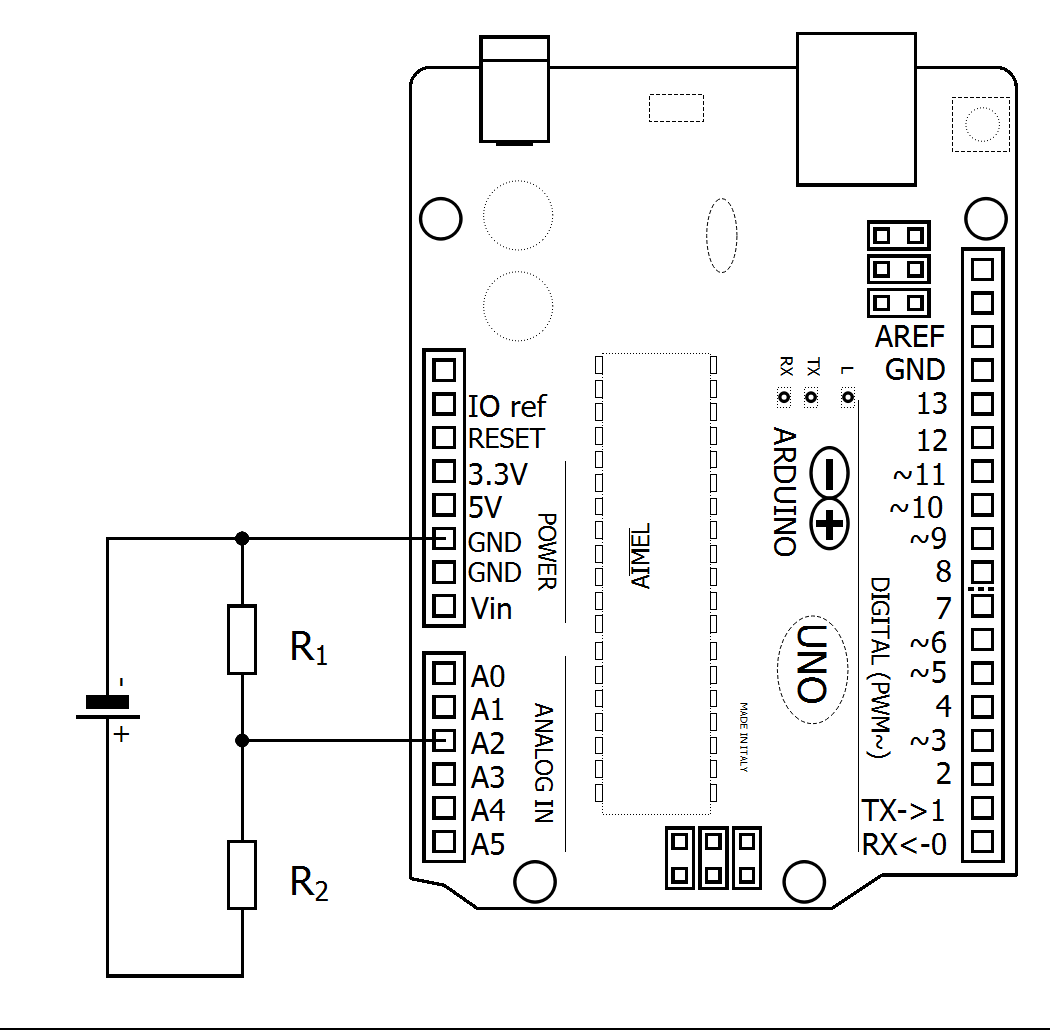
\includegraphics[width=0.4\textwidth]{../Zeichnungen/schaltplan-spannungsmessung.png}
		\end{wrapfigure}
		Mit der rechts abgebildeten Schaltung sollen am Arduino Spannungen an der Batterie bis zu $\SI{15}{\volt}$ gemessen werden.
		\begin{enumerate}[label=\alph*),itemsep=0mm,parsep=0mm]
			\item Nenne mögliche, sinnvolle Größen für die Widerstände $R_1$ und $R_2$.
			\item Im analogen Eingang A2 wird ein Wert von 789 gemessen. Berechne die Spannung an der Batterie.
		\end{enumerate}
	\end{aufgabe}
	
	\bigskip
	\emph{Lösung:}
	\begin{enumerate}[label=\alph*),itemsep=0mm,parsep=0mm]
		\item Die Widerstände sollten recht groß sein und im Verhältnis 1 zu 2 stehen, damit die Spannung in A0 5\,V nicht überschreitet. Ein geeignetes Beispiel wäre $R_1=\SI{10}{\kilo\ohm}$ und $R_2=\SI{20}{\kilo\ohm}$.
		\item Die Spannung an $R_1$ wird in A2 gemessen. Sie beträgt:
		\begin{equation*}
			U_1=\frac{789}{1023}\cdot \SI{5}{\volt} \approx \SI{3,86}{\volt}.
		\end{equation*}
		Da sich die Spannung entsprechend des Verhältnisses der Widerstände aufteilt, ist die Spannung an $R_2$ doppelt so groß wie $U_1$ ($U_2\approx \SI{7,71}{\volt}$) und die Gesamtspannung drei Mal so groß wie $U_1$ (oder die Summe der beiden Spannungen; $U_{ges}\approx \SI{11,58}{\volt}$).
	\end{enumerate}
	
	\newpage
	\begin{aufgabe} \emph{Potentiometer}
		
		\begin{enumerate}[label=\alph*), itemsep=0mm]
			\item Erläutere die Funktionsweise eines Potentiometers und nenne ein Einsatzbeispiel.
			\item Skizziere, wie man ein Potentiometer am Arduino anschließt.
			\item Ein Potentiometer hat einen Gesamtwiderstand von $R_{ges}=\SI{10}{\kilo\ohm}$. Der mittlere Kontakt wird im analogen Eingang A0 ausgelesen und liefert einen Analogwert von 824. Berechne, wie groß die Teilwiderstände sind. 
		\end{enumerate}
	\end{aufgabe}
	\vspace{-0.5\baselineskip}
	\emph{Lösung:}
	\vspace{-0.5\baselineskip}
	\begin{enumerate}[label=\alph*), itemsep=0mm]
		\item Ein Potentiometer besteht aus zwei Teilwiderständen, die in Reihe geschaltet sind. Die Größe der Teilwiderstände kann zum Beispiel durch Drehen variiert werden, während der Gesamtwiderstand immer konstant bleibt. Indem man die Größe eines Teilwiderstands (oder der daran abfallenden Spannung) als Eingangssignal für die Helligkeit einer Lampe nutzt, kann man eine Lampe dimmen.
		\item \begin{figure}[H]
			\centering
			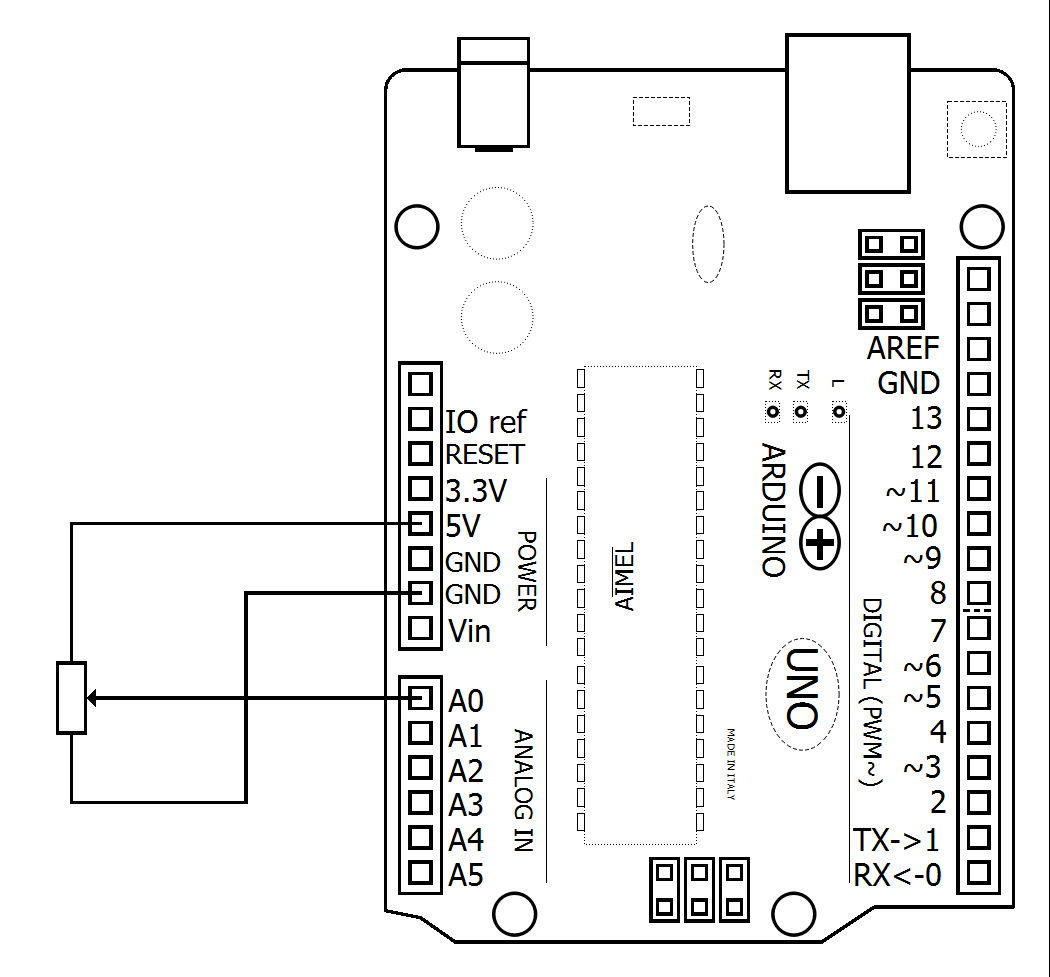
\includegraphics[width=0.35\textwidth]{../Zeichnungen/schaltplan-poti-an-arduino.png}
		\end{figure}
		
		\item Am Widerstand $R_1$ zwischen A0 und GND fällt die Spannung $U_1=\frac{824}{1023}\cdot \SI{5}{\volt}\approx \SI{4,03}{\volt}$ ab. Damit verbleibt für die Spannung $U_2$ am Widerstand $R_2$ zwischen A0 und 5V ein Wert von $U_2 = \SI{5}{\volt}-\SI{4,03}{\volt} = \SI{0,97}{\volt}$.
		
		Im Spannungsteiler gilt:
		
		\begin{equation*}
			\frac{R_{ges}}{U_{ges}} = \frac{R_1}{U_1} = \frac{R_2}{U_2}.
		\end{equation*}
		
		Einsetzen der bekannten Werte liefert:
		\begin{align*}
			R_1 &= \frac{R_{ges}}{U_{ges}} \cdot U_1 = \frac{\SI{10}{\kilo\ohm}}{\SI{5}{\volt}} \cdot \SI{4,03}{\volt} \approx \SI{8,05}{\kilo\ohm}, \\
			R_2 &= \frac{R_{ges}}{U_{ges}} \cdot U_2 = \frac{\SI{10}{\kilo\ohm}}{\SI{5}{\volt}} \cdot \SI{0,97}{\volt} \approx \SI{1,95}{\kilo\ohm}. \\
		\end{align*}
		
		Alternativ: $R_2=\SI{10}{\kilo\ohm} - R_1 = \SI{1,95}{\kilo\ohm}$.
	\end{enumerate}
	
	\begin{aufgabe} \emph{Dimmbarer Lautsprecher}
		
		\begin{wrapfigure}{r}{0.4\textwidth}
			\centering
			\vspace{-1\baselineskip}
			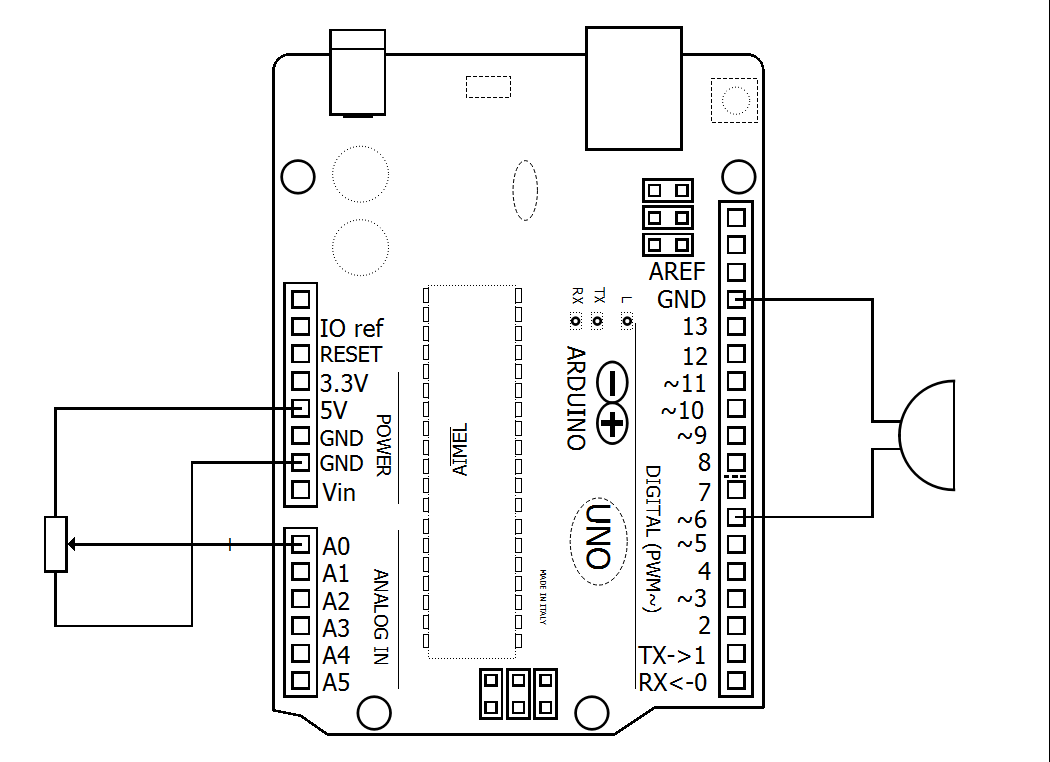
\includegraphics[width=0.4\textwidth]{../Zeichnungen/schaltplan-dimmbarer-lautsprecher.png}
		\end{wrapfigure}
		Der Schaltplan rechts zeigt ein Potentiometer, dessen mittlerer Kontakt am analogen Eingang A0 eines Arduino angeschlossen ist. Auf der anderen Seite ist ein Piezo-Summer an Digitalpin 6 des Arduino angeschlossen.
		
		Entwickle mit den unten abgebildeten Befehlen ein Programm, das dafür sorgt, dass die Lautstärke des Piezo-Summers durch das Potentiometer gedimmt werden kann. Das Programm soll in einem Struktogramm dokumentiert werden.
		
		\begin{figure}[H]
			\centering
			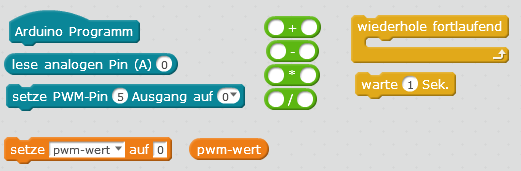
\includegraphics[width=0.8\textwidth]{../pics/befehle-fuer-dimmbaren-lautsprecher.png}
		\end{figure}
	\end{aufgabe}
	
	\bigskip
	\emph{Lösung:}
	
	\begin{tikzpicture}
	\draw (0,0) rectangle (14,3);
	\draw (0.5,0) -- (0.5,2) -- (14,2);
	\draw (0.5,1) rectangle (14,2);
	\draw (0.5,0) rectangle (14,1);
	\node at (6.5,2.5) {wiederhole fortlaufend};
	\node at (6.5,1.5) {setze pwm-wert auf (((lese analogen Pin (A)0) /1023)*255)};
	\node at (6.5,0.5) {setze PWM-Pin 6 Ausgang auf pwm-wert};
	\end{tikzpicture}
	
	\begin{aufgabe} \emph{LDR und NTC - Basics}
		
		\medskip
		\begin{minipage}{0.59\textwidth}
			\begin{enumerate}[label=\alph*), itemsep=0mm, parsep=0mm]
				\item Nenne jeweils einen Einsatzzweck für einen LDR und einen NTC.
				\item Beschreibe das Widerstandsverhalten eines LDR (eines NTC), wenn sich die Helligkeit (die Temperatur) verringert.
				\item Ein NTC ist in einem Spannungsteiler mit einem Festwiderstand mit $R_F=\SI{10}{\kilo\ohm}$ am Arduino angeschlossen (s. Schaltplan rechts). Im analogen Eingang A0 wird ein Wert von 643 gemessen. Berechne die Größe des Widerstands des NTC.
			\end{enumerate}
		\end{minipage}
		\hfill
		\begin{minipage}{0.39\textwidth}
			\centering
			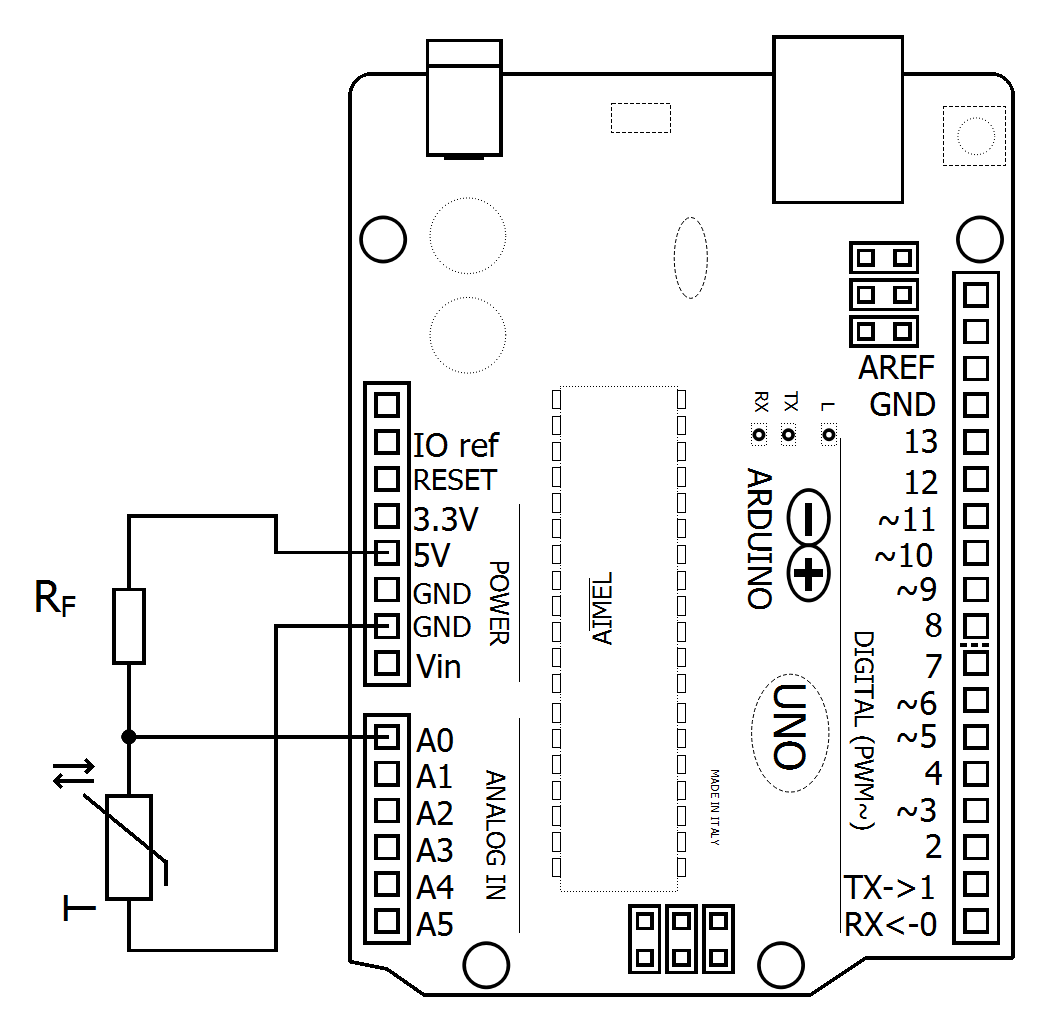
\includegraphics[width=\textwidth]{../Zeichnungen/schaltplan-ntc-an-arduino.png}
		\end{minipage}
		
		\begin{minipage}{0.48\textwidth}
			\begin{enumerate}[label=\alph*), itemsep=0mm, parsep=0mm]
				\setcounter{enumi}{3}
				\item Die Tabelle unten zeigt für den verwendeten NTC, welche Widerstandswerte $R$ zu welcher Temperatur $T$ gehören. Bestimme mit Hilfe einer quadratischen Regression einen funktionalen Zusammenhang zwischen $R$ und $T$ und berechne damit die Temperatur, die zum Widerstandswert aus Aufgabenteil c) gehört.
			\end{enumerate}
		\end{minipage}
		\hfill
		\begin{minipage}{0.48\textwidth}
			\begin{tcolorbox}[sharp corners]
				\begin{minipage}{0.48\textwidth}
					R/T No. \textbf{8307}
					
					\bigskip
					Widerstand
					
					bei $\ang{25}$: 
					
					$R_{25}=\SI{10}{\kilo\ohm}$.
					
					\vspace{2\baselineskip}
				\end{minipage}
				\hfill
				\begin{minipage}{0.48\textwidth}
					\begin{tabular}{l | l }
						T (C) & $R_T/R_{25}$ \\ \hline
						5.0 & 2.252 \\ \hline
						10.0 & 1.8216 \\ \hline
						15.0 & 1.4827 \\ \hline
						20.0 & 1.2142 \\ \hline
						25.0 & 1.0000 \\ \hline
						30.0 & 0.82818 \\ \hline
					\end{tabular}
				\end{minipage}
			\end{tcolorbox}
		\end{minipage}
	\end{aufgabe}
	
	\bigskip
	\emph{Lösung:}
	
	\begin{enumerate}[label=\alph*), itemsep=0mm, parsep=0mm]
		\item Mit einem LDR lässt sich die Helligkeit messen. Dies kann zum Beispiel genutzt werden, um die Bildschirmbeleuchtung eines Handys automatisch an die Umgebungshelligkeit anzupassen, um eine Wetterstation zu bauen, um Straßenlaternen zu steuern etc.
		
		Mit einem NTC lässt sich die Temperatur messen. Damit kann zum Beispiel ein Fieberthermometer gebaut werden, eine Wetterstation oder der NTC wird als Sensor für einen 3D-Drucker genutzt.
		\item Je größer die Helligkeit ist, desto kleiner ist der Widerstand eines LDR.
		
		Je größer die Temperatur ist, desto kleiner ist der Widerstand eines NTC.
		\item Die Spannung am NTC beträgt $U_{NTC}= \frac{643}{1023}\cdot \SI{5}{\volt} \approx \SI{3,14}{\volt}$.
		
		Im Spannungsteiler gilt:
		\begin{equation*}
			\frac{R_F}{U_F} = \frac{R_{NTC}}{U_{NTC}} \Rightarrow R_{NTC} = \frac{R_F}{U_F} \cdot U_{NTC} = \frac{\SI{10}{\kilo\ohm}}{\SI{5}{\volt}-\SI{3,14}{\volt}} \cdot \SI{3,14}{\volt} \approx \SI{16,92}{\kilo\ohm}.
		\end{equation*}
		\item Für die Regression sollten die Widerstandsverhältnisse in Widerstandswerte umgerechnet werden:
		
		\smallskip
		\begin{tabular}{l | l }
			T (C) & $R_T (\SI{}{\kilo\ohm})$ \\ \hline
			5.0 & 22.52 \\ \hline
			10.0 & 18.216 \\ \hline
			15.0 & 14.827 \\ \hline
			20.0 & 12.142 \\ \hline
			25.0 & 10.000 \\ \hline
			30.0 & 8.2818 \\ \hline
		\end{tabular}
		
		\smallskip
		Eine quadratische Regression liefert: 
		
		$y=0,06855\cdot x^2 -3,83443\cdot x + 56,7452$ 
		
		bzw. 
		
		$T(R)=0,06855\cdot R^2 -3,83443\cdot R + 56,7452$ (T in $\SI{}{\celsius}$, R in $\SI{}{\kilo\ohm}$).
		
		Einsetzen von $R=\SI{16,92}{\kilo\ohm}$ liefert:
		
		$T(\SI{16,92}{\kilo\ohm}) \approx \SI{11,5}{\celsius} $.
		
		An der untersuchten Stelle ist es also ungefähr $\SI{11}{\celsius}$ bis $\SI{12}{\celsius}$ kalt.
	\end{enumerate}
	
	\newpage
	\begin{aufgabe} \emph{LDR komplex}
		
		\medskip
		\begin{minipage}{0.5\textwidth}
			Für ein \href{https://www.el-voss.de/?p=159}{Moorhuhn-Lasertag} kann man zwei gleichartige LDR in Reihe schalten und wie abgebildet am Arduino anschließen. Jeder LDR soll zu einem Moorhuhn gehören. Durch Einlesen des Wertes in A0 soll ermittelt werden, welches Moorhuhn vom Laser getroffen wurde.
			
			\begin{enumerate}[label=\alph*), itemsep=0mm, parsep=0mm]
				\item Erläutere, welche Auswirkung der Laser beim Treffen eines LDR auf die Widerstände und die Spannungen hat.
				\item Erkläre, welcher Wert sich in A0 näherungsweise einstellen sollte, wenn gerade keiner der beiden LDR getroffen ist.
			\end{enumerate}
		\end{minipage}
		\hfill
		\begin{minipage}{0.48\textwidth}
			\centering
			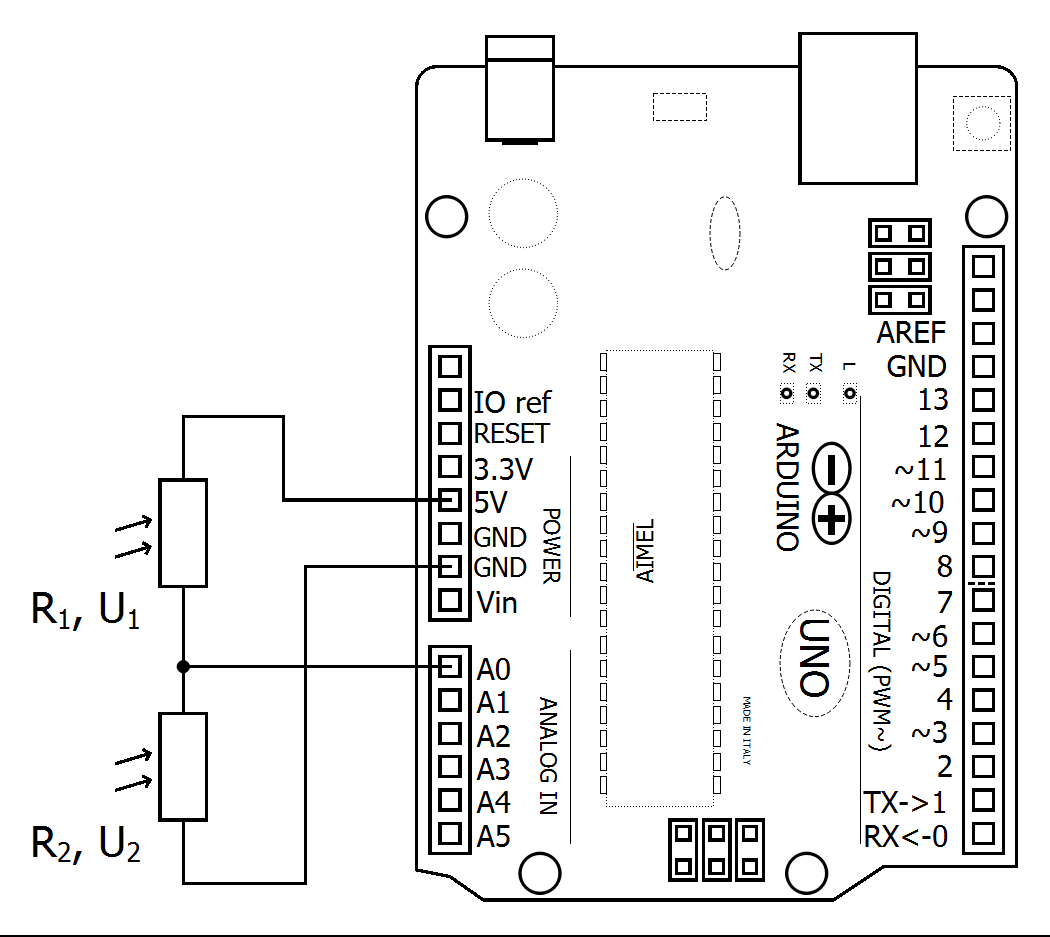
\includegraphics[width=\textwidth]{../Zeichnungen/schaltplan-ldr-in-reihe.png}
		\end{minipage}
		
		\begin{enumerate}[label=\alph*), itemsep=0mm, parsep=0mm]
			\setcounter{enumi}{2}
			\item Entwickle mithilfe der unten abgebildeten Befehle ein Programm, das auf dem seriellen Monitor ausgibt, welches Moorhuhn (welcher LDR) getroffen wurde. Das Programm soll als Struktogramm dargestellt werden.
		\end{enumerate}
		
		\begin{figure}[H]
			\centering
			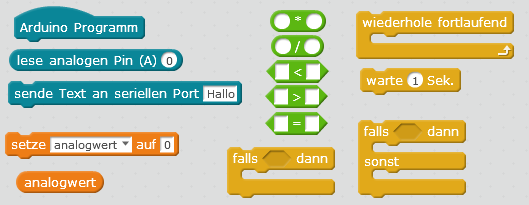
\includegraphics[width=0.8\textwidth]{../pics/befehle-fuer-ldr-in-reihe.png}
		\end{figure}
	\end{aufgabe}

	\bigskip
	\emph{Lösung:}
	
	\begin{enumerate}[label=\alph*), itemsep=0mm, parsep=0mm]
		\item Wenn der Laserpointer auf LDR1 trifft, nimmt sein Widerstand stark ab, während der Widerstand von LDR2 gleich bleibt. Dadurch nimmt auch die Spannung an LDR1 stark ab. Weil die Gesamtspannung immer 5\,V betragen muss, nimmt also die Spannung an LDR2 stark zu. (Diese wird in A0 gemessen.)
		
		Wenn der Laserpointer auf LDR2 trifft, nimmt sein Widerstand stark ab, während der Widerstand von LDR1 gleich bleibt. Dadurch nimmt auch die Spannung an LDR2 stark ab. Weil die Gesamtspannung immer 5\,V betragen muss, nimmt also die Spannung an LDR1 stark zu. 
		
		\item Wenn keiner der LDR getroffen ist, haben beide ungefähr den gleichen Widerstand. Die Spannung, die an den LDR abfällt, sollte also jeweils ca. 2,5\,V betragen. Dies entspricht einem Analogwert von $\frac{\SI{2,5}{\volt}}{\SI{5}{\volt}}\cdot 1023 =512$.
		
		\item Folgendes Programm liefert eine Lösung, die noch als Struktogramm dargestellt werden muss.
		
		\begin{figure}[H]
			\centering
			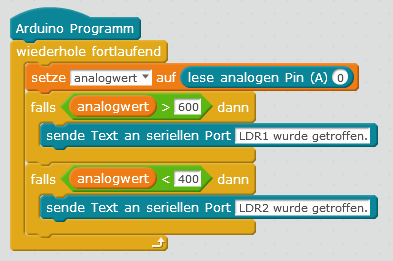
\includegraphics[width=0.5\textwidth]{../pics/programm-ldr-in-reihe.png}
		\end{figure}
	\end{enumerate}
	
	\begin{aufgabe} \emph{Transistor}
		
		\begin{wrapfigure}{r}{0.4\textwidth}
			\centering
			\vspace{-\baselineskip}
			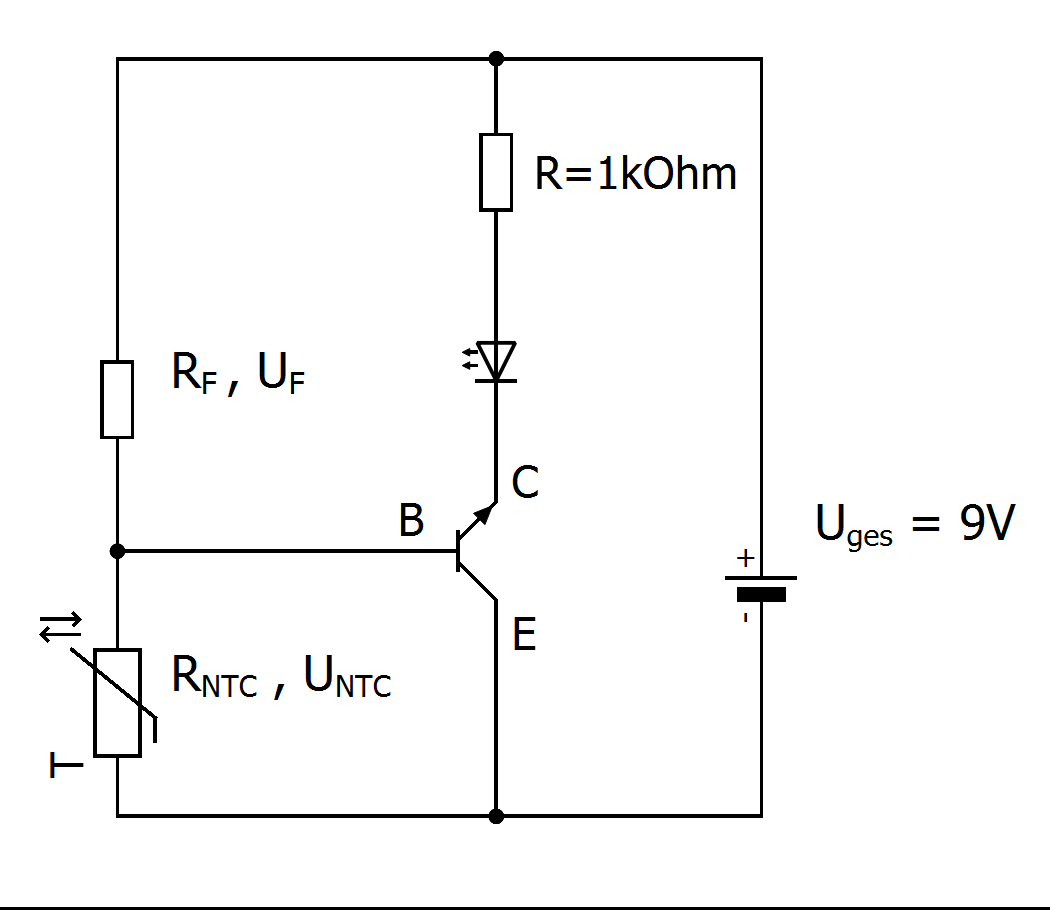
\includegraphics[width=0.4\textwidth]{../Zeichnungen/schaltplan-transistor-und-ntc.png}
		\end{wrapfigure}
		Der Schaltplan rechts zeigt eine Transistor-Grundschaltung, in der ein Spannungsteiler mit einem Festwiderstand $R_F$ und ein NTC mit Widerstand $R_{NTC}$ verbaut ist. In der folgenden Tabelle ist festgehalten, bei welcher Temperatur der NTC welchen Widerstand hat.
		
		\medskip
		\begin{tabular}{l|l|l|l}
			$T$ in $\SI{}{\celsius}$ & 25 & 20 & 15 \\ \hline
			$R$ in $\SI{}{\kilo\ohm}$ & 10 & 12,1 & 14,8 \\
		\end{tabular}
		
		\medskip
		Bestimme die Größe von $R_F$ so, dass der Transistor bei $\SI{25}{\celsius}$ ($\SI{20}{\celsius}$, $\SI{15}{\celsius}$) schaltet.
		
		\emph{Hinweis:} Der Transistor schaltet bei einer Spannung $U_{BE} = \SI{0,7}{\volt}$.
	\end{aufgabe}
	
	\bigskip
	\emph{Lösung:}
	
	Schalten bei $\SI{25}{\celsius}$:
	
	Im Spannungsteiler von Festwiderstand und NTC gilt die Spannungsteilerformel:
	
	\begin{equation*}
		\frac{R_F}{U_F} = \frac{R_{NTC}}{U_{NTC}}.
	\end{equation*}
	
	Bei $\SI{25}{\celsius}$ beträgt der Widerstand des NTC (siehe Tabelle) $R(\SI{25}{\celsius}) = \SI{10}{\kilo\ohm} $.
	
	Die Spannung am NTC ist die gleiche, die zwischen Basis und Emitter abfällt. Das heißt, der Transistor schaltet, wenn $U_{NTC} = U_{BE} = \SI{0,7}{\volt}$. Von der Gesamtspannung $U_{ges}=\SI{9}{\volt}$ bleiben für die Spannung am Festwiderstand dann noch $U_F=\SI{8,3}{\volt}$ übrig.
	
	Umformen und Einsetzen liefert:
	
	\begin{equation*}
		R_F = \frac{R_{NTC}}{U_{NTC}} \cdot U_F = \frac{\SI{10}{\kilo\ohm}}{\SI{0,7}{\volt}} \cdot \SI{8,3}{\volt} \approx \SI{119}{\kilo\ohm}.
	\end{equation*}
	
	\newpage
	Für die anderen Temperaturen müssen nur die Werte für den Widerstand des NTC angepasst werden:
	
	Schalten bei $\SI{20}{\celsius}$:
	
	\begin{equation*}
	R_F = \frac{R_{NTC}}{U_{NTC}} \cdot U_F = \frac{\SI{12,1}{\kilo\ohm}}{\SI{0,7}{\volt}} \cdot \SI{8,3}{\volt} \approx \SI{143}{\kilo\ohm}.
	\end{equation*}
	
	Schalten bei $\SI{15}{\celsius}$:
	
	\begin{equation*}
	R_F = \frac{R_{NTC}}{U_{NTC}} \cdot U_F = \frac{\SI{14,8}{\kilo\ohm}}{\SI{0,7}{\volt}} \cdot \SI{8,3}{\volt} \approx \SI{175}{\kilo\ohm}.
	\end{equation*}
	
\end{document}



%%%%%%%%%%%%%%%%%%%%%%%%%%%%%%%%%%%%%%%%%%%%%%%%%%%%%%%%%%%%%%%%%%%%%%%%%%%%%%%%%%%%%%%%%%%%%%%%%%

\begin{minipage}{0.49\textwidth}
	\centering
	Für die LEDs an Pin 1 bis 5:
	
	\begin{tikzpicture}
	\draw (0,0) rectangle (7,7);
	\draw (0.5,0) rectangle (7,6);
	\draw (0.5,5) rectangle (7,6);
	\draw (1,0) rectangle (7,4);
	\draw (1,3) rectangle (7,4);
	\draw (1,2) rectangle (7,3);
	\draw (1,1) rectangle (7,2);
	\node at (3.5,6.5) {wiederhole fortlaufend};
	\node at (3.5,5.5) {setze p auf 1};
	\node at (3.5,4.5) {wiederhole 5 mal};
	\node at (3.5,3.5) {setze Pin p auf HIGH};
	\node at (3.5,2.5) {warte 1 Sekunde};
	\node at (3.5,1.5) {setze Pin p auf LOW};
	\node at (3.5,0.5) {ändere p um 1};
	\end{tikzpicture}
	
	Alternativ:
	
	\begin{tikzpicture}
	\draw (0,0) rectangle (7,7);
	\draw (0.5,0) rectangle (7,6);
	\draw (0.5,5) rectangle (7,6);
	\draw (1,0) rectangle (7,4);
	\draw (1,3) rectangle (7,4);
	\draw (1,2) rectangle (7,3);
	\draw (1,1) rectangle (7,2);
	\node at (3.5,6.5) {wiederhole fortlaufend};
	\node at (3.5,5.5) {setze p auf 1};
	\node at (3.5,4.5) {wiederhole bis p = 6};
	\node at (3.5,3.5) {setze Pin p auf HIGH};
	\node at (3.5,2.5) {warte 1 Sekunde};
	\node at (3.5,1.5) {setze Pin p auf LOW};
	\node at (3.5,0.5) {ändere p um 1};
	\end{tikzpicture}
\end{minipage}
\hfill
\begin{minipage}{0.49\textwidth}
	\centering
	
	Für die LEDs 2, 4, 6, 8:
	
	\begin{tikzpicture}
	\draw (0,0) rectangle (7,7);
	\draw (0.5,0) rectangle (7,6);
	\draw (0.5,5) rectangle (7,6);
	\draw (1,0) rectangle (7,4);
	\draw (1,3) rectangle (7,4);
	\draw (1,2) rectangle (7,3);
	\draw (1,1) rectangle (7,2);
	\node at (3.5,6.5) {wiederhole fortlaufend};
	\node at (3.5,5.5) {setze p auf 2};
	\node at (3.5,4.5) {wiederhole 4 mal};
	\node at (3.5,3.5) {setze Pin p auf HIGH};
	\node at (3.5,2.5) {warte 1 Sekunde};
	\node at (3.5,1.5) {setze Pin p auf LOW};
	\node at (3.5,0.5) {ändere p um 2};
	\end{tikzpicture}
	
	\vspace{13.5\baselineskip}
\end{minipage}	